\documentclass{beamer}
%\documentclass[trans]{beamer}

\usetheme[%pageofpages=/,% String used between the current page and the total page count.
%bullet=circle,% Use circles instead of squares for bullets.
titleline=true,% Show a line below the frame title.
alternativetitlepage=true,% Use the fancy title page.
%titlepagelogo=logo-polito,% Logo for the first page.
]{Torino} 

\newcommand{\code}[1]{\textbf{#1}}

\usepackage{parcolumns}
\usepackage{listings} 
\usepackage{subfig}
\author{Lasse Folger}
\title{\huge Lazy Software Transactional Memory}
\subtitle{Master Thesis}
\date{05.04.2017}

\lstset{escapeinside=!!}
\begin{document}
  \begin{frame}[t,plain]
    \titlepage
  \end{frame}
  
  
  \begin{frame}
    \frametitle{Motivation}
    \lstinputlisting{ressources/accountMVar.hs}
  \end{frame}
  
  \begin{frame}[fragile]
    \frametitle{MVar}
    \fboxsep=0pt
    \noindent
    \begin{minipage}[t]{0.48\linewidth}
      Thread 1:
            \begin{figure}
       \begin{lstlisting}[frame=single]
transfer acc1 acc2 50
       \end{lstlisting}
      \end{figure}
\end{minipage}%
    \hfill%
    \begin{minipage}[t]{0.48\linewidth}
      Thread 2:      
      \begin{figure}
       \begin{lstlisting}[frame=single]
transfer acc2 acc1 50
       \end{lstlisting}
      \end{figure}
    \end{minipage}
\end{frame}

  \begin{frame}[fragile]
    \frametitle{MVar}
    \fboxsep=0pt
    \noindent
    \begin{minipage}[t]{0.48\linewidth}
      Thread 1:
            \begin{figure}
       \begin{lstlisting}[frame=single]
a1 <- takeMVar acc1 
a2 <- takeMVar acc2 
writeMVar acc1 (a1 - 50)
writeMVar acc2 (a2 + 50)
       \end{lstlisting}
      \end{figure}
\end{minipage}%
    \hfill%
    \begin{minipage}[t]{0.48\linewidth}
      Thread 2:      
      \begin{figure}
       \begin{lstlisting}[frame=single]
b1 <- takeMVar acc2 
b2 <- takeMVar acc1 
writeMVar acc2 (b1 - 50)
writeMVar acc1 (b2 + 50)
       \end{lstlisting}
      \end{figure}
    \end{minipage}
    \vfill
    \pause
    $\Rightarrow$ Deadlock
\end{frame}
  
  \begin{frame}
    \frametitle{Use Transactions}
    \lstinputlisting{ressources/accountTVar.hs}   
  \end{frame}
  
  \begin{frame}[fragile]
    \frametitle{TVar}
    \fboxsep=0pt
    \noindent
    \begin{minipage}[t]{0.48\linewidth}
      Thread 1:
      \begin{figure}
       \begin{lstlisting}[frame=single]
atomically $ 
  transfer acc1 acc2 50
       \end{lstlisting}
      \end{figure}
    \end{minipage}%
    \hfill%
    \begin{minipage}[t]{0.48\linewidth}
      Thread 2:
      \begin{figure}
       \begin{lstlisting}[frame=single]
atomically $ 
  transfer acc2 acc1 50
       \end{lstlisting}
      \end{figure}
    \end{minipage}
    \vfill
    \pause
    $\Rightarrow$ works fine, because transactions provide ACI(D) properties
\end{frame}
%%%%%%%%%%%%%%%%%%%%%%%%%%%%
%%%Current Implementation%%%
%%%%%%%%%%%%%%%%%%%%%%%%%%%%
  \begin{frame}
    \frametitle{Current Implementation (Control.Concurrent.STM)}
    \begin{itemize}\setlength\itemsep{1em}
      \item \textit{writeTVar}, \textit{readTVar} and \textit{newTVar} modify TVars
      \item \textit{retry} and \textit{orElse} alter the control flow
      \item \textit{atomically} executes a transaction 
      \item composition via bind operator (or do)
    \end{itemize}
  \end{frame}
  
  \begin{frame}
   \frametitle{Transactional Log}
   \begin{itemize}\setlength\itemsep{1em}
    \item one log per transaction
    \item three elements per log entry
          \begin{itemize}
           \item \code{TVar}
           \item \code{expectedValue}
           \item \code{currentValue}
          \end{itemize}
   \end{itemize}
  \end{frame}
  
  \begin{frame}
   \frametitle{Modify Operations}
   \begin{itemize}\setlength\itemsep{1em}
    \item \textbf{newTVar}: creates a new, initialized TVar 
    \item \textbf{writeTVar}: updates \textit{currentValue} in log entry
    \item \textbf{readTVar}: reads TVar from log or actual TVar
  \end{itemize}
\end{frame}
  
%   \begin{frame}
%    \frametitle{Control Flow Operations}
%    \begin{itemize}\setlength\itemsep{1em}
%     \item \textbf{retry}: suspends until a read TVar is written.
%     \item \textbf{orElse}: takes two transactions
%       \begin{itemize}
%        \item runs the first transaction
%        \item if the first transaction retrys it runs the second transaction
%       \end{itemize}
%   \end{itemize}
%   \end{frame}
%   
  \begin{frame}
   \frametitle{\lstinline{atomically :: STM a -> IO a}}
   \begin{enumerate}\setlength\itemsep{1em}
    \item compute the log
    \item lock TVars
    \item validate the log
    \item if valid then commit
    \item else roll back
   \end{enumerate}
  \end{frame}

  \begin{frame}
   \frametitle{Validation}
    \begin{enumerate}\setlength\itemsep{1em}
%       \item lock the TVars in the read set
      \item compare \textit{expectedValue} to the value in the actual TVar
      \item if all values match return valid 
      \item else return invalid
    \end{enumerate}
  \end{frame}

%%%%%%%%%%%%%%%%%% 
%%%%%Problems%%%%%
%%%%%%%%%%%%%%%%%%

\begin{frame}[fragile]
    \frametitle{Problem}
    \fboxsep=0pt
    \noindent
    \begin{minipage}[t]{0.48\linewidth}
      Thread 1:
    \begin{figure}
     \begin{lstlisting}[frame=single]
a1 <- readTVar acc1
a2 <- readTVar acc2
writeTVar acc1 (a1 - 50)
writeTVar acc2 (a2 + 50)
     \end{lstlisting}
    \end{figure}
    \end{minipage}%
    \hfill%
    \begin{minipage}[t]{0.48\linewidth}
      Thread 2:
    \begin{figure}
     \begin{lstlisting}[frame=single]
b1 <- readTVar acc2
b2 <- readTVar acc1
writeTVar acc2 (b1 - 50)
writeTVar acc1 (b2 + 50)
     \end{lstlisting}
    \end{figure}
    \end{minipage}
\end{frame}


    \begin{frame}[fragile]
    \frametitle{Problem}
    \fboxsep=0pt
    \noindent
    \begin{minipage}[t]{0.48\linewidth}
      Thread 1:
    \begin{figure}
     \begin{lstlisting}[frame=single]
[(acc1, a1, a1-50),
 (acc2, a2, a2+50)]
     \end{lstlisting}
    \end{figure}
    \end{minipage}%
    \hfill%
    \begin{minipage}[t]{0.48\linewidth}
      Thread 2:
    \begin{figure}
     \begin{lstlisting}[frame=single]
[(acc2, b1, b1-50),
 (acc1, b2, b2+50)]
    \end{lstlisting}
    \end{figure}
    \end{minipage}
\end{frame}

\begin{frame}[fragile]
    \frametitle{Problem}
    \fboxsep=0pt
    \noindent
    \begin{minipage}[t]{0.48\linewidth}
      Thread 1:
    \begin{figure}
     \begin{lstlisting}[frame=single]
a1 <- readTVar acc1
a2 <- readTVar acc2
writeTVar acc1 (a1 - 50)
writeTVar acc2 (a2 + 50)
     \end{lstlisting}
    \end{figure}
    \end{minipage}%
    \hfill%
    \begin{minipage}[t]{0.48\linewidth}
      Thread 2:
    \begin{figure}
     \begin{lstlisting}[frame=single]
b1 <- readTVar acc2
b2 <- readTVar acc1
writeTVar acc2 (b1 - 50)
writeTVar acc1 (b2 + 50)
     \end{lstlisting}
    \end{figure}
    \end{minipage}
    \vfill
    $\Rightarrow$ either sequential or one transaction is rolled back
\end{frame}


\begin{frame}
 \frametitle{Critical TVar}
   \begin{itemize}\setlength\itemsep{1em}
    \item Critical between read and commit
    \item modifications to critical TVars cause rollback
   \end{itemize}
   \pause
   \vfill
   $\Rightarrow$ minimize the time TVars are critical 
\end{frame}


  
  \begin{frame}
   \frametitle{Critical TVar}
   \begin{figure}
    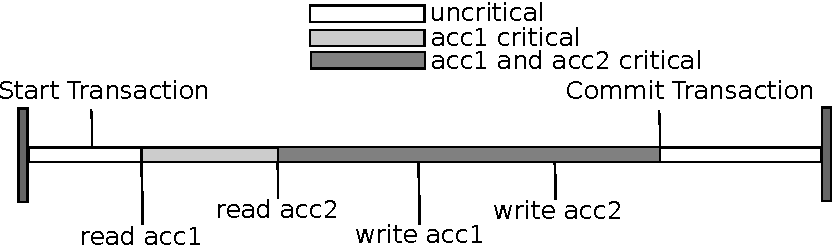
\includegraphics[scale=0.7]{ressources/CriticalValue.pdf}
   \end{figure}
   \end{frame}

\begin{frame}[fragile]
\frametitle{Idea}
\begin{lstlisting}
transfer = do 
  a1 <- readTVar acc2
  writeTVar acc2 (a1 - 50)
  a2 <- readTVar acc1
  writeTVar acc1 (a2 + 50)
\end{lstlisting}
\end{frame}
  
     
  \begin{frame}
   \frametitle{Critical TVar}
   \begin{figure}
    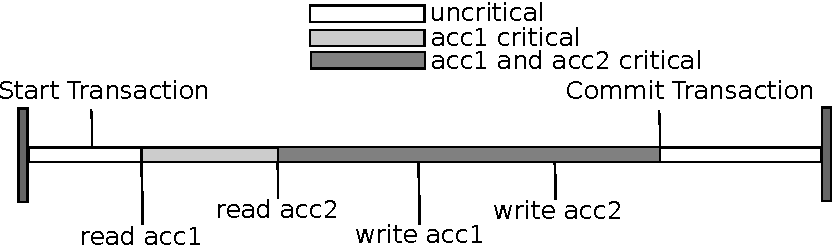
\includegraphics[scale=0.7]{ressources/CriticalValue.pdf}
   \end{figure}
   \begin{figure}
    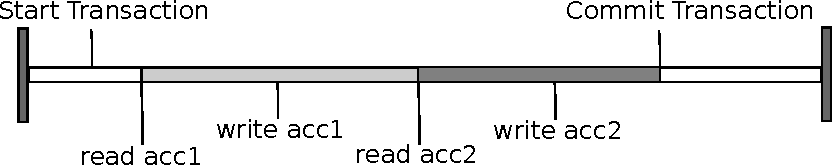
\includegraphics[scale=0.7]{ressources/CriticalValue2.pdf}
   \end{figure}
   \end{frame}

\begin{frame}
 \frametitle{Idea}
 \begin{itemize}\setlength\itemsep{1em}
  \item delay the evaluation of \code{readTVar} to commit phase
  \item no TVars is critical at all  
  \item \code{writeTVar} does not need the value in the computation phase
 \end{itemize}
\end{frame}
  
\begin{frame}[fragile]
   \frametitle{Idea does not work}
   \begin{lstlisting}[language=Haskell]
limitedTransfer src dst am = do
   a1 <- readTVar src
   if a1 < am
     then return ()
     else do a2 <- readTVar  dst
             writeTVar src (a1 - am)
             writeTVar dst (a2 + am)
   \end{lstlisting}
   \vfill
   $\Rightarrow$ idea does not work because the value is needed.
\end{frame}

%   \begin{frame}[fragile]
%    \frametitle{Problem}
%       \begin{itemize}\setlength\itemsep{1em}
%        \item\lstinline[language=Haskell]{(>>=) :: STM a -> (a -> STM b) -> STM b}
%        \item Bind extracts the value from the STM context
%        \item STM no longer controls this value.
%        \item Need another Typeclass than Monad
%       \end{itemize}
% \end{frame}
% 
% 
%   \begin{frame}[fragile]
%    \frametitle{Applicative}
%       \begin{itemize}\setlength\itemsep{1em}
%        \item Applicative is less powerfull than Monad
%        \item\lstinline[language=Haskell]{(<*>) :: STM (a -> b) -> STM a -> STM b}
%        \item The value can be modified without leaving the STM context
%       \end{itemize}
% \end{frame}

%%%%%%%%%%%%%%%%%%%%%%%%%%
%%%%%What I have done%%%%%
%%%%%%%%%%%%%%%%%%%%%%%%%%
%   
%   \begin{frame}
%    \frametitle{Project}
%    \begin{itemize}\setlength\itemsep{1em}
%     \item Improved a pure Haskell implementation
%     \item Direct notification
%     \item Explicit, ordered locking
%     \item Optimisations
%    \end{itemize}
%   \end{frame}


  \begin{frame}
   \frametitle{Solution}
   \begin{itemize}\setlength\itemsep{1em}
    \item delay evaluation as far as possible
    \item evaluate them just before they are needed..
    \item ..or in the commit phase
   \end{itemize}
  \end{frame}


  \begin{frame}
   \frametitle{When is a value needed?}
   \begin{itemize}\setlength\itemsep{1em}
    \item branch conditions
       \begin{itemize}
        \item if-then-else
        \item case
        \item patternmatching
        \item guards
       \end{itemize}
    \item IO-actions $\Rightarrow$ not allowed in STM
   \end{itemize}
  \end{frame}

  \begin{frame}
  \frametitle{Implementation}
  \begin{itemize}\setlength\itemsep{1em}
   \item pure Haskell implementation
   \item state monad
   \item computation phase modifies the state 
   \item commit phase uses state to validate and commit
  \end{itemize}
  \end{frame}
  
  \begin{frame}
  \frametitle{UnsafePerformIO}
  \begin{itemize}\setlength\itemsep{1em}
   \item pure Haskell implementation
   \item state monad
   \item computation phase modifies the state 
   \item commit phase uses state to validate and commit
  \end{itemize}
  \end{frame}
  

%   \begin{frame}[fragile]
%    \frametitle{\lstinline[language=Haskell]{writeTVar :: TVar a -> STM a -> STM ()}}
%    \begin{lstlisting}[language=Haskell]
% example = do
%    writeTVar t2 (readTVar t1)
%    a <- readTVar t2
%    if a ...
%    \end{lstlisting}
% \end{frame}

  
  \begin{frame}
   \frametitle{New Combinators}
   \begin{itemize}\setlength\itemsep{1em}
    \item \lstinline[language=Haskell]{(<*>) :: STM (a -> b) -> STM a -> STM b}
    \item \lstinline[language=Haskell]{(<**>) :: STM a -> STM (a -> b) -> STM b}
%     \item \lstinline[language=Haskell]{(*>) :: STM a -> STM b -> STM b}
    \item \lstinline[language=Haskell]{(**>) :: STM a -> (STM a  -> STM b) -> STM b}
    \item \lstinline[language=Haskell]{(>>=) :: STM a -> (a -> STM b) -> STM b}
    \item \lstinline[language=Haskell]{(>>) :: STM a -> STM b -> STM b}
   \end{itemize}
  \end{frame}

  
  \begin{frame}[fragile]
    \frametitle{New Transfer}
    \lstinputlisting{ressources/accountTVar2.hs}
\end{frame}
  
 
  \begin{frame}[fragile]
    \frametitle{Problem solved}
    \fboxsep=0pt
    \noindent
    \begin{minipage}[t]{0.48\linewidth}
      Thread 1:
      \begin{figure}
       \begin{lstlisting}[frame=single]
atomically $ 
  transfer acc1 acc2 50
       \end{lstlisting}
      \end{figure}
    \end{minipage}%
    \hfill%
    \begin{minipage}[t]{0.48\linewidth}
      Thread 2:
      \begin{figure}
       \begin{lstlisting}[frame=single]
atomically $ 
  transfer acc2 acc1 50
       \end{lstlisting}
      \end{figure}
    \end{minipage}
    \vfill
    $\Rightarrow$ no more rollback
\end{frame}
  
  
%%%%%%%%%%%%%%%%%%%%%%
%%%%%Future Work%%%%%%
%%%%%%%%%%%%%%%%%%%%%%
  \begin{frame}
   \frametitle{Todo}
   \begin{itemize}\setlength\itemsep{1em}
    \item Reduce the number of combinators
    \item Change writeTVars type and use ApplicativeDo
    \item \textbf{But} it extracts the Value from STM context
    \item investigate other problems:
      \begin{itemize}
        \item Branch condition is not changed by TVar modification
        \item Recomputation of values which did not change
      \end{itemize}
   \end{itemize}
  \end{frame}

  \begin{frame}[fragile]
    \frametitle{Unnecessary Recomputation}
    \begin{lstlisting}[language=Haskell]
     transaction = do
       lmitedTransfer acc1 acc2 50
       limtedTransfer acc3 acc4 100
    \end{lstlisting}
    \vfill
    If one transfer is invalidated, both are recomputed
\end{frame}


\begin{frame}
 \frametitle{Questions about...}
 \begin{itemize}\setlength\itemsep{1em}
  \item ...Control.Concurrent.STM?
  \item ...rollback avoidance?
  \item ...unnecessary recomputation?
  \item ...something else?
 \end{itemize}

\end{frame}


  
\end{document}



